\begin{figure}[!tb]
  \centering
 
  \begin{subfigure}{1.0\textwidth}
\centering

    \begin{tabular}{@{}c@{}}
    \resizebox{0.5\linewidth}{!}{
      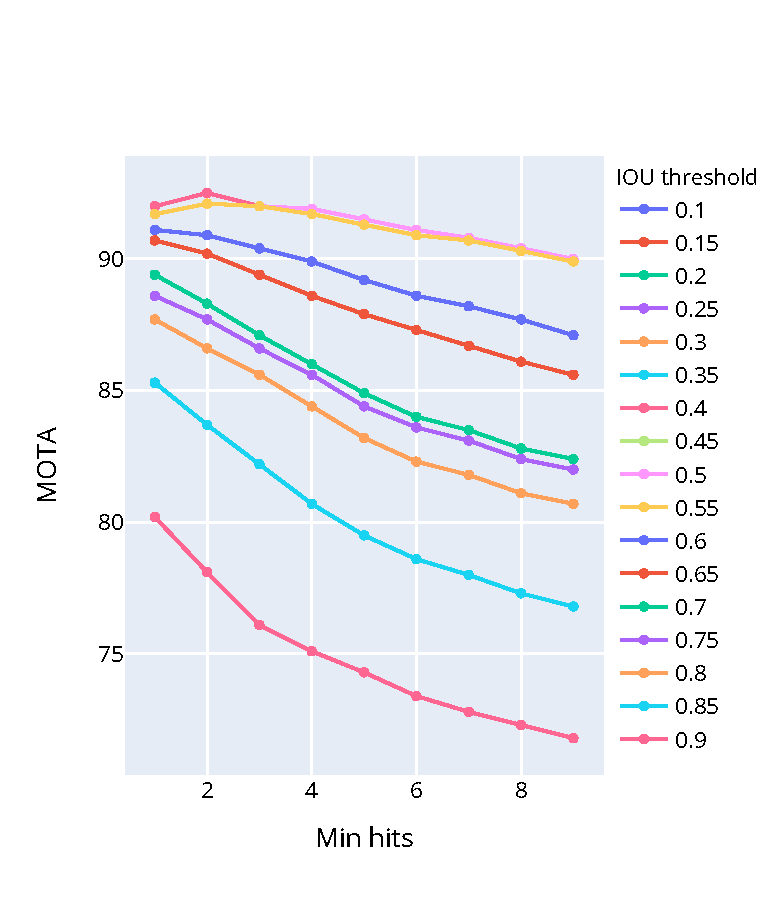
\includegraphics{img/optimizing_tracker_0.pdf}}
    \end{tabular}\qquad
    \resizebox{0.4\linewidth}{!}{
    \begin{tabular}{rrrr}
    \toprule
     Max age &  Min hits & IOU threshold &  MOTA \\
    \midrule
           1 &         2 &       0.10 & 92.50 \\
           1 &         2 &       0.15 & 92.50 \\
           1 &         2 &       0.20 & 92.50 \\
           1 &         2 &       0.25 & 92.50 \\
           1 &         2 &       0.30 & 92.50 \\
           1 &         2 &       0.35 & 92.50 \\
           1 &         2 &       0.40 & 92.50 \\
    \bottomrule
    \end{tabular}
    }
    
    \caption{Tuning parameters by maximizing MOTA on "person" object class.}
    \label{fig:optimizing_tracker_0}
  \end{subfigure}
 
    \bigskip
 
  \begin{subfigure}{1.0\linewidth}
    \centering
    
    \begin{tabular}{@{}c@{}}
    \resizebox{0.5\linewidth}{!}{
      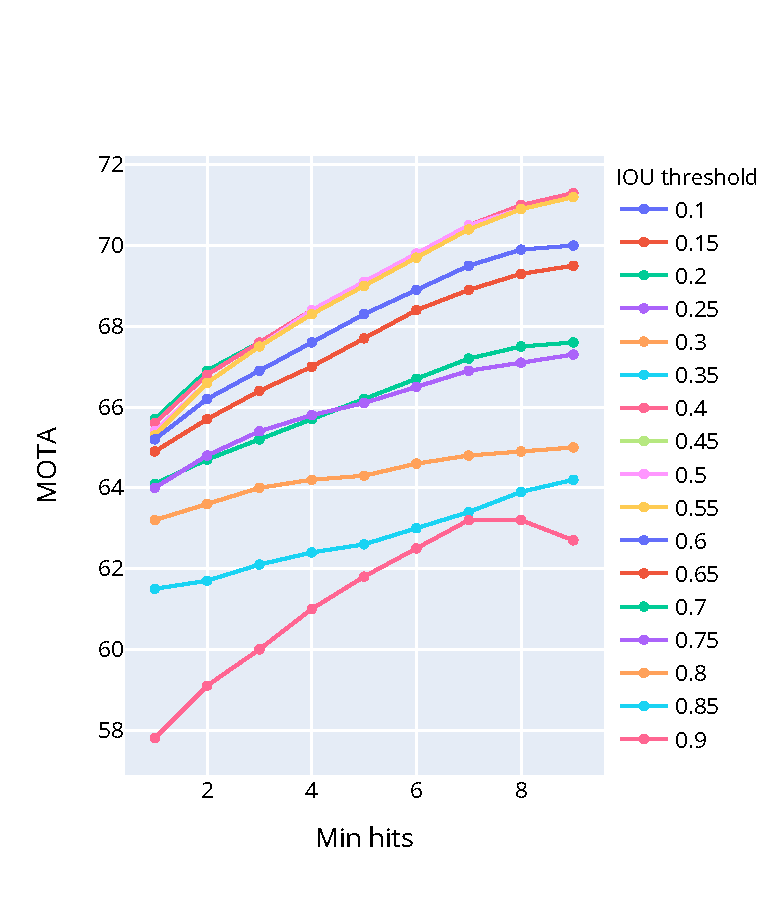
\includegraphics{img/optimizing_tracker_all.pdf}}
    \end{tabular}\qquad
    \resizebox{0.4\linewidth}{!}{
    \begin{tabular}{rrrr}
    \toprule
     Max age &  Min hits &  IOU threshold &  MOTA \\
    \midrule
           1 &         9 &       0.10 & 71.30 \\
           1 &         9 &       0.15 & 71.30 \\
           1 &         9 &       0.20 & 71.30 \\
           1 &         9 &       0.25 & 71.30 \\
           1 &         9 &       0.30 & 71.30 \\
           1 &         9 &       0.35 & 71.30 \\
           1 &         9 &       0.40 & 71.30 \\
    \bottomrule
    \end{tabular}
    }
    
    \caption{Tuning parameters by maximizing MOTA on "all" object classes.}
    \label{fig:optimizing_tracker_all}
  \end{subfigure}
  

  \caption[Optimizing SORT by maximizing MOTA score on "person" and "all" object classes]
  {Optimizing SORT by maximizing MOTA score on "person" and "all" object classes.}
  \label{fig:optimizing_tracker} % label should be placed below caption
\end{figure}